% \documentclass[10pt, aspectratio=169, handout]{beamer}
\documentclass[10pt, aspectratio=169, handout, dvipsnames]{beamer}
\usefonttheme{professionalfonts}

\mode<presentation>
{
  \usetheme{Berkeley}
  \usecolortheme{beaver}
  \usefonttheme{default}
  \setbeamertemplate{navigation symbols}{}
  \setbeamertemplate{caption}[numbered]
} 

\setbeamertemplate{footline}{%
  \leavevmode%
  \hbox{%
    \begin{beamercolorbox}[wd=.85\paperwidth,ht=2.5ex,dp=1ex,left]{author in head/foot}%
      \usebeamerfont{author in head/foot}Digital Signal Processing, Fall 2025%
    \end{beamercolorbox}%
    \begin{beamercolorbox}[wd=.15\paperwidth,ht=2.5ex,dp=1ex,right]{date in head/foot}%
      \hspace*{0.5em}\insertframenumber{} / \inserttotalframenumber\hspace*{0.5em}%
    \end{beamercolorbox}%
  }%
  \vskip0pt%
}

\usepackage[english]{babel}
\usepackage[utf8x]{inputenc}
\usepackage{tikz}
\usepackage{pgfplots}
\usepackage{array}
\usepackage{makecell}
\usepackage{verbatim}
\usepackage{graphicx}
\usepackage{subcaption}
\usepackage{amsfonts}
\usepackage{amsmath}
\usepackage{bm}
\usepackage{epstopdf}
\captionsetup{compatibility=false}

\usetikzlibrary{calc}
\usetikzlibrary{pgfplots.fillbetween, backgrounds}
\usetikzlibrary{positioning}
\usetikzlibrary{pgfplots.groupplots}
\usetikzlibrary{plotmarks}
\usetikzlibrary{calc}
\usetikzlibrary{patterns}
\usetikzlibrary{decorations.pathreplacing}




% % \usepackage{tikz}
% \usetikzlibrary{external}
% \tikzexternalize[prefix=figures/]
% \tikzset{external/system call={pdflatex \tikzexternalcheckshellescape -halt-on-error -interaction=batchmode -jobname "\image" "\texsource"}}


\usepgfplotslibrary{groupplots}
\pgfplotsset{compat=newest} 




\usepackage{ifthen}
\newboolean{showresults}
\setboolean{showresults}{false}

\usepackage{hyperref}
\hypersetup{
    colorlinks=true,
    linkcolor=blue,
    filecolor=magenta,      
    urlcolor=cyan,
}

\title[ECEN 463/863]{The z-Transform}
\author{Maxx Seminario}
\institute{University of Nebraska-Lincoln}
\date{October 13, 2025}

\begin{document}



\begin{frame}
  \titlepage
\end{frame}

\section{Introduction}

\begin{frame}{Overview: The z-Transform}
\begin{itemize}
    \item \textbf{Motivation}: 
    \begin{itemize}
        \item Fourier transform doesn't converge for all sequences
        \item Need a more general transform that encompasses broader class of signals
        \item z-transform notation often more convenient for analysis
    \end{itemize}
    
    \item \textbf{Key Relationships}:
    \begin{itemize}
        \item z-transform for discrete-time $\leftrightarrow$ Laplace transform for continuous-time
        \item Similar relationship to corresponding Fourier transforms
        \item Fourier transform is special case: $X(e^{j\omega}) = X(z)|_{z=e^{j\omega}}$
    \end{itemize}
    
    \item \textbf{Today's Topics}:
    \begin{itemize}
        \item Definition and convergence of z-transform
        \item Region of Convergence (ROC) properties
        \item Examples of common z-transform pairs
        \item Properties of rational z-transforms
    \end{itemize}
\end{itemize}
\end{frame}

\section{z-Transform Definition}

\begin{frame}{The z-Transform}
\textbf{Definition}:
\begin{align}
    X(z) &= \sum_{n=-\infty}^{\infty} x[n]z^{-n} \quad \text{(bilateral z-transform)}
\end{align}

where $z$ is a complex variable.

\vspace{0.3cm}
\textbf{z-Transform Operator}:
\[
    \mathcal{Z}\{x[n]\} = \sum_{n=-\infty}^{\infty} x[n]z^{-n} = X(z)
\]

\vspace{0.3cm}
\textbf{Notation}: $x[n] \overset{\mathcal{Z}}{\longleftrightarrow} X(z)$

\vspace{0.3cm}
\textbf{One-sided z-Transform}:
\[
    X(z) = \sum_{n=0}^{\infty} x[n]z^{-n} \quad \text{(unilateral z-transform)}
\]

\end{frame}

\begin{frame}{Relationship to Fourier Transform}
\begin{columns}
\begin{column}{0.5\textwidth}
\textbf{Complex Variable in Polar Form}:
% \[
%     z = re^{j\omega}
% \]

\vspace{-0.6cm}
% \textbf{z-Transform becomes}:
\begin{align}
     z &= re^{j\omega} \\
    X(re^{j\omega}) &= \sum_{n=-\infty}^{\infty} x[n](re^{j\omega})^{-n} \\
    &= \sum_{n=-\infty}^{\infty} (x[n]r^{-n})e^{-j\omega n}
\end{align}

% \vspace{0.3cm}
\textbf{Interpretation}:
\begin{itemize}
    \item z-transform = Fourier transform of $x[n]r^{-n}$
    \item For $r = 1$ (unit circle): $X(e^{j\omega})$ = Fourier transform
    \item $|z| = 1$ defines the unit circle in z-plane
\end{itemize}
\end{column}
\begin{column}{0.5\textwidth}
\begin{center}
\begin{tikzpicture}[scale=1.5]
    \draw[->] (-2,0) -- (2,0) node[right] {Re};
    \draw[->] (0,-2) -- (0,2) node[above] {Im};
    \draw[thick,blue] (0,0) circle (1);
    \draw[->,red,thick] (0,0) -- (0.707,0.707) node[midway,left] {$z = e^{j\omega}$};
    \node at (0.3,1.3) [blue] {Unit circle};
    \node at (1.1,0.5) {$\omega$};
    \draw[dashed] (0,0) -- (1,0);
\end{tikzpicture}
\end{center}
\end{column}
\end{columns}
\end{frame}

\section{Region of Convergence}

\begin{frame}{Region of Convergence (ROC)}
\begin{columns}
\begin{column}{0.5\textwidth}
\textbf{Definition}: Set of values of $z$ for which the z-transform converges

\vspace{0.3cm}
\textbf{Convergence Condition}:
\[
    |X(re^{j\omega})| \leq \sum_{n=-\infty}^{\infty} |x[n]r^{-n}| < \infty
\]

\vspace{0.3cm}
\textbf{Key Properties}:
\begin{itemize}
    \item Convergence depends only on $|z| = r$
    \item ROC consists of a ring in z-plane: $r_R < |z| < r_L$
    \item If ROC includes unit circle $\Rightarrow$ Fourier transform exists
\end{itemize}
\end{column}
\begin{column}{0.5\textwidth}
\begin{center}
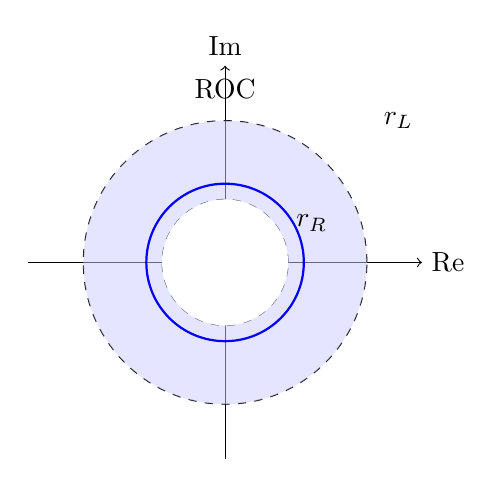
\begin{tikzpicture}[scale=1]
    \draw[->] (-2.5,0) -- (2.5,0) node[right] {Re};
    \draw[->] (0,-2.5) -- (0,2.5) node[above] {Im};
    \draw[dashed] (0,0) circle (0.8);
    \draw[dashed] (0,0) circle (1.8);
    \fill[blue!20,opacity=0.5] (0,0) circle (1.8);
    \fill[white] (0,0) circle (0.8);
    \draw[thick,blue] (0,0) circle (1);
    \node at (2.2,1.8) {$r_L$};
    \node at (1.1,0.5) {$r_R$};
    \node at (0,2.2) {ROC};
\end{tikzpicture}
\end{center}
\end{column}
\end{columns}
\end{frame}
\begin{frame}{Example: Right-Sided Exponential}
\begin{columns}
\begin{column}{0.5\textwidth}
\textbf{Signal}: $x[n] = a^n u[n]$

% \vspace{0.3cm}
\textbf{z-Transform}:
\begin{align}
    X(z) &= \sum_{n=0}^{\infty} a^n z^{-n} \\
    &= \sum_{n=0}^{\infty} (az^{-1})^n
\end{align}

% \vspace{0.3cm}
\textbf{Convergence}: 
\begin{itemize}
    \item Requires $|az^{-1}| < 1$ 
    \item Therefore: $|z| > |a|$
\end{itemize}

% \vspace{0.3cm}
\textbf{Closed Form}:
\[
    X(z) = \frac{1}{1 - az^{-1}} = \frac{z}{z - a} \quad \text{for } |z| > |a|
\]

\end{column}
\begin{column}{0.5\textwidth}
\begin{center}
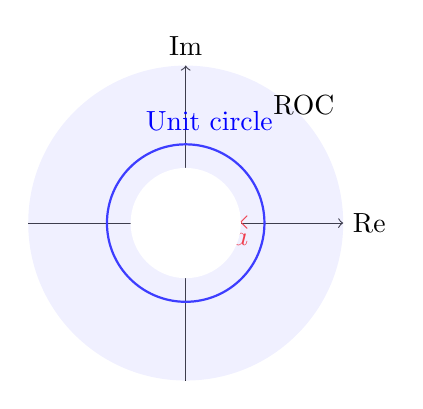
\begin{tikzpicture}[scale=1]
    \draw[->] (-2,0) -- (2,0) node[right] {Re};
    \draw[->] (0,-2) -- (0,2) node[above] {Im};
    \draw[thick,blue] (0,0) circle (1);
    \draw[red,thick] (0.7,0) node {$\times$} node[below] {$a$};
    \draw[green,thick] (0,0) node {$\circ$};
    \fill[blue!20,opacity=0.3] (0,0) circle (2);
    \fill[white] (0,0) circle (0.7);
    \node at (1.5,1.5) {ROC};
    \node at (0.3,1.3) [blue] {Unit circle};
\end{tikzpicture}
\end{center}
\end{column}
\end{columns}
\end{frame}

\begin{frame}{Example: Left-Sided Exponential}
\begin{columns}
\begin{column}{0.5\textwidth}
\textbf{Signal}: $x[n] = -a^n u[-n-1]$

% \vspace{0.3cm}
\textbf{z-Transform}:
\begin{align}
    X(z) &= -\sum_{n=-\infty}^{-1} a^n z^{-n} \\
    &= 1 - \sum_{n=0}^{\infty} (a^{-1}z)^n
\end{align}

% \vspace{0.3cm}
\textbf{Convergence}: 
\begin{itemize}
    \item Requires $|a^{-1}z| < 1$ 
    \item Therefore: $|z| < |a|$
\end{itemize}

% \vspace{0.3cm}
\textbf{Closed Form}:
\[
    X(z) = \frac{1}{1 - az^{-1}} = \frac{z}{z - a} \quad \text{for } |z| < |a|
\]


\vspace{0.2cm}
\textbf{Note}: Same expression, different ROC!
\end{column}
\begin{column}{0.5\textwidth}
\begin{center}
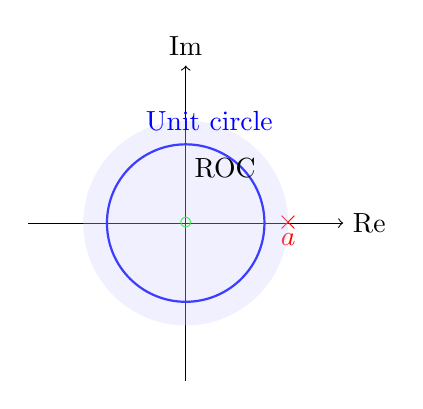
\begin{tikzpicture}[scale=1]
    \draw[->] (-2,0) -- (2,0) node[right] {Re};
    \draw[->] (0,-2) -- (0,2) node[above] {Im};
    \draw[thick,blue] (0,0) circle (1);
    \draw[red,thick] (1.3,0) node {$\times$} node[below] {$a$};
    \draw[green,thick] (0,0) node {$\circ$};
    \fill[blue!20,opacity=0.3] (0,0) circle (1.3);
    \node at (0.5,0.7) {ROC};
    \node at (0.3,1.3) [blue] {Unit circle};
\end{tikzpicture}
\end{center}
\end{column}
\end{columns}
\end{frame}





\section{Properties of ROC}

\begin{frame}{Properties of the ROC}
\begin{enumerate}
    \item \textbf{General Form}: $0 \leq r_R < |z| < r_L \leq \infty$ (annulus)
    
    \item \textbf{Fourier Transform}: Exists iff ROC includes unit circle
    
    \item \textbf{Poles}: ROC cannot contain any poles
    
    \item \textbf{Finite-Duration}: ROC is entire z-plane except possibly $z=0$ or $z=\infty$
    
    \item \textbf{Right-Sided}: ROC extends outward from outermost pole
    
    \item \textbf{Left-Sided}: ROC extends inward from innermost pole
    
    \item \textbf{Two-Sided}: ROC is a ring bounded by poles
    
    \item \textbf{Connected Region}: ROC must be connected
\end{enumerate}
\end{frame}

\begin{frame}{ROC for Different Sequence Types}
\begin{center}
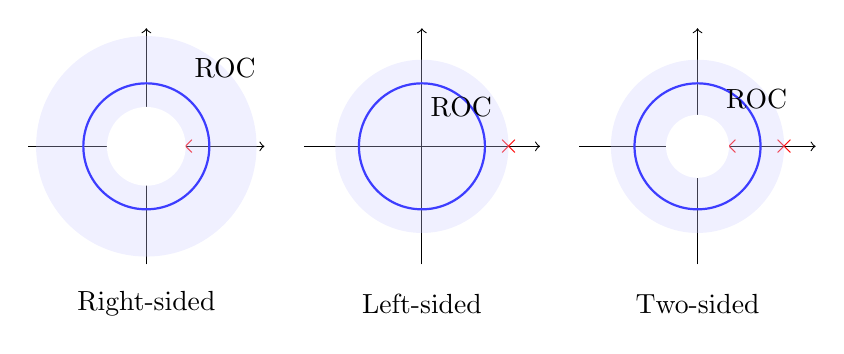
\begin{tikzpicture}
    % Right-sided
    \begin{scope}[shift={(0,0)}]
        \draw[->] (-1.5,0) -- (1.5,0);
        \draw[->] (0,-1.5) -- (0,1.5);
        \draw[thick,blue] (0,0) circle (0.8);
        \draw[red,thick] (0.5,0) node {$\times$};
        \fill[blue!20,opacity=0.3] (0,0) circle (1.4);
        \fill[white] (0,0) circle (0.5);
        \node at (0,-2) {Right-sided};
        \node at (1,1) {ROC};
    \end{scope}
    
    % Left-sided
    \begin{scope}[shift={(3.5,0)}]
        \draw[->] (-1.5,0) -- (1.5,0);
        \draw[->] (0,-1.5) -- (0,1.5);
        \draw[thick,blue] (0,0) circle (0.8);
        \draw[red,thick] (1.1,0) node {$\times$};
        \fill[blue!20,opacity=0.3] (0,0) circle (1.1);
        \node at (0,-2) {Left-sided};
        \node at (0.5,0.5) {ROC};
    \end{scope}
    
    % Two-sided
    \begin{scope}[shift={(7,0)}]
        \draw[->] (-1.5,0) -- (1.5,0);
        \draw[->] (0,-1.5) -- (0,1.5);
        \draw[thick,blue] (0,0) circle (0.8);
        \draw[red,thick] (0.4,0) node {$\times$};
        \draw[red,thick] (1.1,0) node {$\times$};
        \fill[blue!20,opacity=0.3] (0,0) circle (1.1);
        \fill[white] (0,0) circle (0.4);
        \node at (0,-2) {Two-sided};
        \node at (0.75,0.6) {ROC};
    \end{scope}
\end{tikzpicture}
\end{center}
\end{frame}


\begin{frame}{Example: Sum of Two Exponentials}
\begin{columns}
\begin{column}{0.5\textwidth}
\textbf{Signal}: 
\[x[n] = \left(\frac{1}{2}\right)^n u[n] + \left(-\frac{1}{3}\right)^n u[n]\]

% \vspace{0.3cm}
\textbf{z-Transform} (by linearity):
\begin{align}
    X(z) &= \frac{1}{1 - \frac{1}{2}z^{-1}} + \frac{1}{1 + \frac{1}{3}z^{-1}} \\
    &= \frac{2z(z - \frac{1}{12})}{(z - \frac{1}{2})(z + \frac{1}{3})}
\end{align}

% \vspace{0.3cm}
\textbf{ROC}: Intersection of individual ROCs
\begin{itemize}
    \item First term: $|z| > \frac{1}{2}$
    \item Second term: $|z| > \frac{1}{3}$
    \item Combined: $|z| > \frac{1}{2}$
\end{itemize}
\end{column}
\begin{column}{0.5\textwidth}
\begin{center}
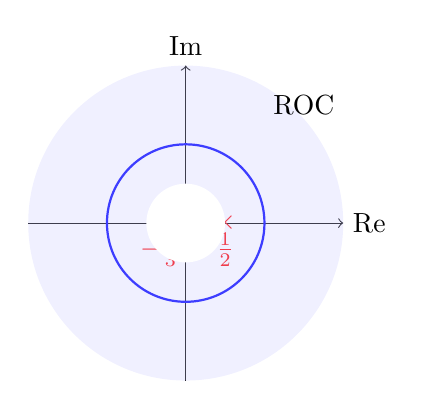
\begin{tikzpicture}[scale=1]
    \draw[->] (-2,0) -- (2,0) node[right] {Re};
    \draw[->] (0,-2) -- (0,2) node[above] {Im};
    \draw[thick,blue] (0,0) circle (1);
    \draw[red,thick] (0.5,0) node {$\times$} node[below] {$\frac{1}{2}$};
    \draw[red,thick] (-0.33,0) node {$\times$} node[below] {$-\frac{1}{3}$};
    \draw[green,thick] (0.083,0) node {$\circ$};
    \fill[blue!20,opacity=0.3] (0,0) circle (2);
    \fill[white] (0,0) circle (0.5);
    \node at (1.5,1.5) {ROC};
\end{tikzpicture}
\end{center}
\end{column}
\end{columns}
\end{frame}



\begin{frame}{Example: Two-Sided Exponential}
\begin{columns}
\begin{column}{0.5\textwidth}
\textbf{Signal}: 
\[x[n] = \left(-\frac{1}{3}\right)^n u[n] - \left(\frac{1}{2}\right)^n u[-n-1]\]

% \vspace{0.2cm}
\textbf{z-Transform}:
\[X(z) = \frac{2z(z - \frac{1}{12})}{(z - \frac{1}{2})(z + \frac{1}{3})}\]

% \vspace{0.2cm}
\textbf{ROC}: 
\begin{itemize}
    \item First term (right-sided): $|z| > \frac{1}{3}$
    \item Second term (left-sided): $|z| < \frac{1}{2}$
    \item Combined: $\frac{1}{3} < |z| < \frac{1}{2}$
\end{itemize}

% \vspace{0.2cm}
\textbf{Note}: ROC doesn't include unit circle 
$\Rightarrow$ no Fourier transform
\end{column}
\begin{column}{0.5\textwidth}
\begin{center}
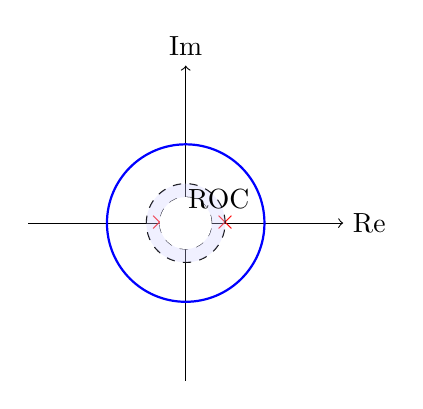
\begin{tikzpicture}[scale=1]
    \draw[->] (-2,0) -- (2,0) node[right] {Re};
    \draw[->] (0,-2) -- (0,2) node[above] {Im};
    \draw[thick,blue] (0,0) circle (1);
    \draw[red,thick] (0.5,0) node {$\times$};
    \draw[red,thick] (-0.33,0) node {$\times$};
    \draw[green,thick] (0.083,0) node {$\circ$};
    \draw[dashed] (0,0) circle (0.33);
    \draw[dashed] (0,0) circle (0.5);
    \fill[blue!20,opacity=0.3] (0,0) circle (0.5);
    \fill[white] (0,0) circle (0.33);
    \node at (0.42,0.3) {ROC};
\end{tikzpicture}
\end{center}
\end{column}
\end{columns}
\end{frame}

\begin{frame}{Finite-Length Sequences}
\begin{columns}
\begin{column}{0.5\textwidth}
\textbf{Example}: $x[n] = a^n, \quad 0 \leq n \leq N-1$

% \vspace{0.3cm}
\textbf{z-Transform}:
\begin{align}
    X(z) &= \sum_{n=0}^{N-1} a^n z^{-n} \\
    &= \frac{1 - (az^{-1})^N}{1 - az^{-1}} \\
    &= \frac{z^N - a^N}{z^{N-1}(z - a)}
\end{align}

% \vspace{0.3cm}
\textbf{Zeros}: 
\[z_k = ae^{j2\pi k/N}, \quad k = 0, 1, ..., N-1\]

% \vspace{0.3cm}
\textbf{ROC}: Entire z-plane except $z = 0$ 
(assuming $|a| < \infty$)
\end{column}
\begin{column}{0.5\textwidth}
\begin{center}
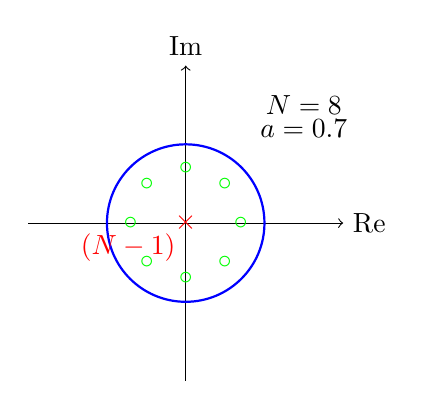
\begin{tikzpicture}[scale=1]
    \draw[->] (-2,0) -- (2,0) node[right] {Re};
    \draw[->] (0,-2) -- (0,2) node[above] {Im};
    \draw[thick,blue] (0,0) circle (1);
    \draw[red,thick] (0,0) node {$\times$} node[below left] {$(N-1)$};
    
    % Draw zeros in a circle
    \foreach \i in {0,1,2,3,4,5,6,7} {
        \draw[green,thick] ({0.7*cos(\i*45)},{0.7*sin(\i*45)}) node {$\circ$};
    }
    
    \node at (1.5,1.5) {$N = 8$};
    \node at (1.5,1.2) {$a = 0.7$};
\end{tikzpicture}
\end{center}
\end{column}
\end{columns}
\end{frame}



\section{Common z-Transform Pairs}

\begin{frame}{Common z-Transform Pairs}
\begin{table}[h]
\centering
\small
\begin{tabular}{|l|l|l|}
\hline
\textbf{Sequence} & \textbf{Transform} & \textbf{ROC} \\
\hline
$\delta[n]$ & $1$ & All $z$ \\
\hline
$u[n]$ & $\frac{1}{1-z^{-1}}$ & $|z| > 1$ \\
\hline
$a^n u[n]$ & $\frac{1}{1-az^{-1}}$ & $|z| > |a|$ \\
\hline
$-a^n u[-n-1]$ & $\frac{1}{1-az^{-1}}$ & $|z| < |a|$ \\
\hline
$na^n u[n]$ & $\frac{az^{-1}}{(1-az^{-1})^2}$ & $|z| > |a|$ \\
\hline
$\cos(\omega_0 n)u[n]$ & $\frac{1-\cos(\omega_0)z^{-1}}{1-2\cos(\omega_0)z^{-1}+z^{-2}}$ & $|z| > 1$ \\
\hline
$\sin(\omega_0 n)u[n]$ & $\frac{\sin(\omega_0)z^{-1}}{1-2\cos(\omega_0)z^{-1}+z^{-2}}$ & $|z| > 1$ \\
\hline
$r^n\cos(\omega_0 n)u[n]$ & $\frac{1-r\cos(\omega_0)z^{-1}}{1-2r\cos(\omega_0)z^{-1}+r^2z^{-2}}$ & $|z| > r$ \\
\hline
\end{tabular}
\end{table}
\end{frame}

\begin{frame}{Rational z-Transforms}
\textbf{General Form}:
\[
    X(z) = \frac{P(z)}{Q(z)} = \frac{b_0 + b_1z^{-1} + ... + b_Mz^{-M}}{1 + a_1z^{-1} + ... + a_Nz^{-N}}
\]

\vspace{0.3cm}
\textbf{Key Points}:
\begin{itemize}
    \item Zeros: roots of $P(z) = 0$
    \item Poles: roots of $Q(z) = 0$
    \item ROC determined by pole locations
    \item Any sum of exponentials $\Rightarrow$ rational z-transform
\end{itemize}

\vspace{0.3cm}
\textbf{Pole-Zero Plot}:
\begin{itemize}
    \item Poles: marked with $\times$
    \item Zeros: marked with $\circ$
    \item Must specify ROC to uniquely determine sequence
\end{itemize}
\end{frame}

\begin{frame}{Example: Multiple ROCs for Same Pole-Zero Pattern}
\textbf{Given}: Poles at $z = a, b, c$ with $|a| < |b| < |c|$

\begin{center}
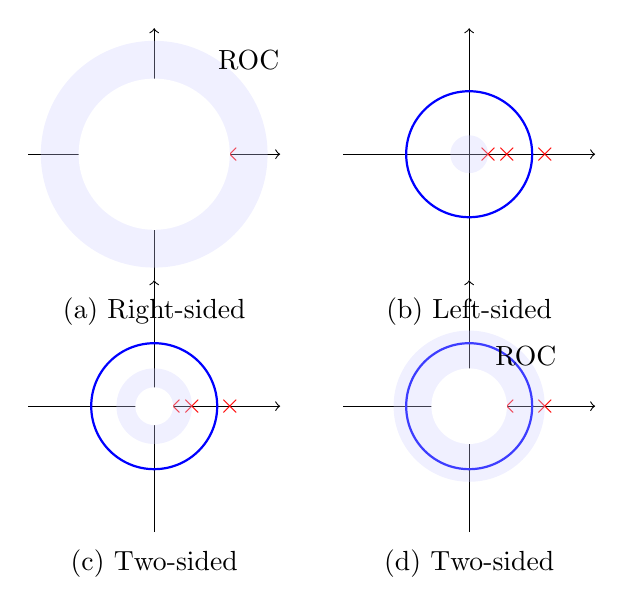
\begin{tikzpicture}[scale=0.8]
    % Plot 1: Right-sided
    \begin{scope}[shift={(0,3)}]
        \draw[->] (-2,0) -- (2,0);
        \draw[->] (0,-2) -- (0,2);
        \draw[thick,blue] (0,0) circle (1);
        \draw[red,thick] (0.3,0) node {$\times$};
        \draw[red,thick] (0.6,0) node {$\times$};
        \draw[red,thick] (1.2,0) node {$\times$};
        \fill[blue!20,opacity=0.3] (0,0) circle (1.8);
        \fill[white] (0,0) circle (1.2);
        \node at (0,-2.5) {(a) Right-sided};
        \node at (1.5,1.5) {ROC};
    \end{scope}
    
    % Plot 2: Left-sided
    \begin{scope}[shift={(5,3)}]
        \draw[->] (-2,0) -- (2,0);
        \draw[->] (0,-2) -- (0,2);
        \draw[thick,blue] (0,0) circle (1);
        \draw[red,thick] (0.3,0) node {$\times$};
        \draw[red,thick] (0.6,0) node {$\times$};
        \draw[red,thick] (1.2,0) node {$\times$};
        \fill[blue!20,opacity=0.3] (0,0) circle (0.3);
        \node at (0,-2.5) {(b) Left-sided};
    \end{scope}
    
    % Plot 3: Two-sided 1
    \begin{scope}[shift={(0,-1)}]
        \draw[->] (-2,0) -- (2,0);
        \draw[->] (0,-2) -- (0,2);
        \draw[thick,blue] (0,0) circle (1);
        \draw[red,thick] (0.3,0) node {$\times$};
        \draw[red,thick] (0.6,0) node {$\times$};
        \draw[red,thick] (1.2,0) node {$\times$};
        \fill[blue!20,opacity=0.3] (0,0) circle (0.6);
        \fill[white] (0,0) circle (0.3);
        \node at (0,-2.5) {(c) Two-sided};
    \end{scope}
    
    % Plot 4: Two-sided 2
    \begin{scope}[shift={(5,-1)}]
        \draw[->] (-2,0) -- (2,0);
        \draw[->] (0,-2) -- (0,2);
        \draw[thick,blue] (0,0) circle (1);
        \draw[red,thick] (0.3,0) node {$\times$};
        \draw[red,thick] (0.6,0) node {$\times$};
        \draw[red,thick] (1.2,0) node {$\times$};
        \fill[blue!20,opacity=0.3] (0,0) circle (1.2);
        \fill[white] (0,0) circle (0.6);
        \node at (0,-2.5) {(d) Two-sided};
        \node at (0.9,0.8) {ROC};
    \end{scope}
\end{tikzpicture}
\end{center}

Only (d) has Fourier transform (ROC includes unit circle)
\end{frame}

\begin{frame}{Stability and Causality}
\textbf{Example}: System with poles at $z = \frac{1}{2}$ and $z = 2$

\begin{center}
\begin{tikzpicture}[scale=1]
    \draw[->] (-2.5,0) -- (2.5,0) node[right] {Re};
    \draw[->] (0,-2) -- (0,2) node[above] {Im};
    \draw[thick,blue] (0,0) circle (1);
    \draw[red,thick] (0.5,0) node {$\times$} node[below] {$\frac{1}{2}$};
    \draw[red,thick] (2,0) node {$\times$} node[below] {$2$};
    \node at (0.3,1.3) [blue] {Unit circle};
\end{tikzpicture}
\end{center}

\textbf{Three possible ROCs}:
\begin{enumerate}
    \item $|z| < \frac{1}{2}$: Left-sided, not stable
    \item $\frac{1}{2} < |z| < 2$: Two-sided, stable, not causal
    \item $|z| > 2$: Right-sided, causal, not stable
\end{enumerate}

\textbf{Key Point}: For this pole configuration, system cannot be both stable AND causal
\end{frame}

\section{Summary}

\begin{frame}{Summary}
\begin{itemize}
    \item \textbf{z-Transform Definition}:
    \begin{itemize}
        \item Generalization of Fourier transform
        \item Power series in complex variable $z$
        \item Reduces to Fourier transform on unit circle
    \end{itemize}
    
    \item \textbf{Region of Convergence}:
    \begin{itemize}
        \item Critical for uniquely specifying sequence
        \item Depends on sequence type (right/left/two-sided)
        \item Cannot contain poles
        \item Must be connected annular region
    \end{itemize}
    
    \item \textbf{Rational z-Transforms}:
    \begin{itemize}
        \item Result from sums of exponentials
        \item Characterized by poles and zeros
        \item ROC determines sequence properties
    \end{itemize}
    
    \item \textbf{Next Time}: z-Transform properties and inverse z-transform
\end{itemize}
\end{frame}

\end{document}